\section{Hyperparameters optimization}\label{sec:mlphyperopt}

In this section I will describe how the optimization of hyperparameters has
been conducted. In the following, I'm not going to optimize the training
algorithm's parameters \idest{\(\mu\), \(\mu_{inc}\), \(\mu_{dec}\), \etc{} of
the Levenberg-Marquardt backpropagation algorithm}, since, during some tests,
they have been found to be not so relevant for the performance of the trained
network: the only effect was the increase/decrease of training time.

The hyperparameters to be optimized are the following:
\begin{itemize}
\item The architecture of the network (then number of hidden layers and the
	number of hidden units in each layer);
\item The selection between the ``Normal'' and ``Windowed'' feature extraction
	methods;
\item The training algorithm.
\end{itemize}

\subsection{Training algorithm and feature extraction meth\-od
selection}\label{subsec:mlphyperopt}

First, I'm going to select the feature extraction method and the training
algorithm for both networks. This task is accomplished by the script
\texttt{mlphyperopt.m}. The scripts makes use of the \code{pretrainingpipeline}
function which builds the base pipeline with all the stages needed to perform
the training of a MLP network \idest{from the \code{preparedata} stage to the
\code{buildfeaturematrix} stage}, using the output of the
\code{selectfeatures} stage \idest{\code{sequentialfs}} as the list of features
to extract. The effective training of the network is performed in the
\code{trainmlp} stage.

The script tries different combinations of training algorithms, feature
extraction methods and number of hidden units (with a single hidden layer). The
exact architecture of the network will be selected afterwards, in
\secref{subsec:mlpbayesopt}.

The list of training algorithms tested is the following:
\begin{description}
\item[trainlm] The Levenberg-Marquardt backpropagation algorithm;
\item[trainbfg] The Broyden-Fletcher-Goldfarb-Shanno quasi-Newton
	backpropagation algorithm;
\item[trainrp] The resilient backpropagation algorithm;
\item[trainscg] The scaled conjugate gradient backpropagation algorithm.
\item[traincgb] The conjugate gradient backpropagation algorithm;
\item[trainoss] The one-step secant backpropagation algorithm;
\item[traingdx] The gradient descent with momentum backpropagation algorithm;
\item[trainbr] The Bayesian regularization backpropagation algorithm.
\end{description}

Each training algorithm is tested with both feature extraction methods.
Moreover, each configuration is tested with different values for the number of
hidden neurons.

The \texttt{mlphyperopt.m} script finally compares the results from each
configuration and prints the best one. The comparison is made on the
performances obtained on the test sets in order to have an unbiased comparison
of the performances.

For algorithm \code{trainbr}, which does not requires a validation set, data
has been partitioned randomly as follows:
\begin{itemize}
\item Training set: \(85\%\) (\(5100\) samples).
\item Test set: \(15\%\) (\(900\) samples).
\end{itemize}
For all the other algorithms, data has been partitioned randomly as follows:
\begin{itemize}
\item Training set: \(70\%\) (\(4200\) samples).
\item Validation set: \(15\%\) (\(900\) samples).
\item Test set: \(15\%\) (\(900\) samples).
\end{itemize}

The results are shown in \lstref{lst:mlphyperopt}. For the estimation of the
ECG's mean, we get the best results using the ``Normal'' feature extraction
method and the Bayesian regularization backpropagation algorithm
(\code{trainbr}). For the estimation of the ECG's standard deviation instead,
we get better results using the ``Windowed'' feature extraction method with the
Levenberg-Marquardt backpropagation algorithm (\code{trainlm}). Also, from the
output, we can have an idea on the sizes of the network architectures needed in
terms of number of hidden units.

\lstinputlisting[language={}, label={lst:mlphyperopt}, caption={Results for the
execution of the \texttt{mlphyperopt.m} script.}]{mlphyperopt.txt}

\subsection{Bayesian optimization of the network
architecture}\label{subsec:mlpbayesopt}

The exact architecture of the two networks is selected using the script
\texttt{mlpbayesopt.m}. This script uses the \texttt{hyperoptmlp} stage that
uses the Bayesian optimization algorithm (\code{bayesopt}) to minimize the
\code{KFoldCVLoss} function which performs a 5-fold cross-validation.
\code{bayesopt} will try different combinations of the 4 parameters that
defines the architecture of the network in an effort to find the best
combination (ranges have been chosen based on the results of the
\code{mlphyperopt.m} script shown in \lstref{lst:mlphyperopt}):
\begin{description}
\item[hiddenLayers] The number of hidden layers. Range:
	\(\interval{1}{3}\).
\item[hiddenUnits1] The number of hidden neurons in the first layer. Range for
	ECG's mean estimation: \(\interval{10}{35}\). Range for ECG's standard
	deviation estimation: \(\interval{30}{150}\).
\item[hiddenUnits2] The number of hidden neurons in the second layer. Range for
	ECG's mean estimation: \(\interval{0}{15}\). Range for ECG's standard
	deviation estimation: \(\interval{0}{50}\).
\item[hiddenUnits3] The number of hidden neurons in the third layer. Range for
	ECG's mean estimation: \(\interval{0}{5}\). Range for ECG's standard
	deviation estimation: \(\interval{0}{15}\).
\end{description}

Each \code{bayesopt} execution evaluates 100 epochs (100 different combinations
of the four parameters). \tableref{table:mlpbayesopt} shows the best
architectures selected for both networks. \figref{fig:mlparches} shows the
chosen architectures in graphical representation.

\begin{table}[hbtp]
	\centering
	\begin{tabular}{|l|c|c|}
		\toprule
		Parameter & \standout{ECG mean} & \standout{ECG stddev} \\
		\midrule
		hiddensLayers & 3 & 2 \\
		hiddensUnits1 & 10 & 31 \\
		hiddensUnits2 & 8 & 30 \\
		hiddensUnits3 & 2 & 0 \\
		\bottomrule
	\end{tabular}
	\caption{Best architectures selected by \code{bayesopt} for the two
	MLPs.}\label{table:mlpbayesopt}
\end{table}

\begin{figure}[htbp]
	\centering
	\begin{subfigure}{\textwidth}
		\centering
		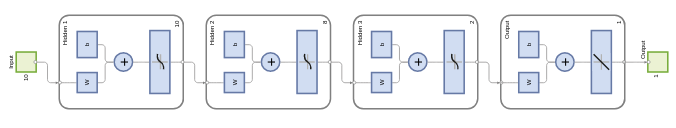
\includegraphics[width=\textwidth]{mlpmeanarch}
		\caption{ECG's mean estimation network
		architecture.}\label{fig:mlpmeanarch}
	\end{subfigure}
	\begin{subfigure}{\textwidth}
		\centering
		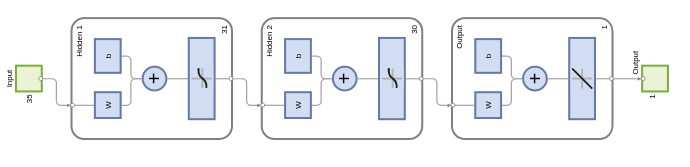
\includegraphics[width=\textwidth]{mlpstdarch}
		\caption{ECG's standard deviation estimation network
		architecture.}\label{fig:mlpstdarch}
	\end{subfigure}
	\caption{Graphical representation of the architectures selected by
	\code{bayesopt}.}\label{fig:mlparches}
\end{figure}
